\documentclass[tikz,border=2pt,11pt]{standalone}
\usetikzlibrary{arrows.meta}
\usetikzlibrary{decorations.pathreplacing}
\usetikzlibrary{calc}
\usetikzlibrary{positioning}
\usepackage{amsmath}
\usepackage{amssymb}
\usepackage{graphicx}
\usepackage{xcolor}
\usepackage{tikz}
\newcommand{\R}{\mathbb R}
\newcommand{\Z}{\mathbb Z}
\newcommand{\N}{\mathbb N}
\newcommand{\F}{\mathbb F}
\newcommand{\E}{\mathbb E}
\newcommand{\Pp}{\mathbb P}
\newcommand{\one}{\mathbf 1}
\newcommand{\Id}{\mathrm{Id}}
\DeclareMathOperator{\TV}{TV}
\DeclareMathOperator{\supp}{supp}
\DeclareMathOperator{\rank}{rank}
\DeclareMathOperator{\diag}{diag}
\DeclareMathOperator{\Span}{span}
\DeclareMathOperator{\KL}{D}
\DeclareMathOperator{\dist}{dist}
\DeclareMathOperator{\diam}{diam}
\DeclareMathOperator{\Lip}{Lip}
\DeclareMathOperator{\tr}{tr}
\DeclareMathOperator{\osc}{osc}
\newcommand{\ip}[2]{\langle #1,#2\rangle}
\begin{document}
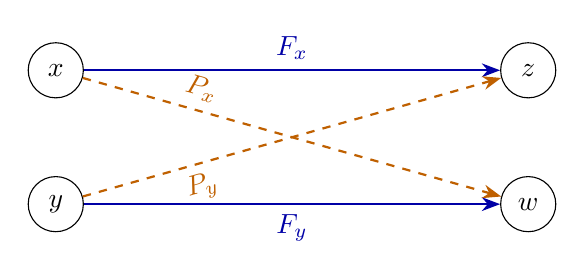
\begin{tikzpicture}[>=Stealth,
 point/.style={circle,draw,minimum size=7mm,inner sep=1pt},
 future/.style={->,thick,blue!65!black},
 past/.style={->,thick,dashed,orange!75!black}]
 \node[point] (x) at (-3,0.85) {$x$};
 \node[point] (y) at (-3,-0.85) {$y$};
 \node[point] (z) at (3,0.85) {$z$};
 \node[point] (w) at (3,-0.85) {$w$};
 \draw[future] (x) -- node[above] {$F_x$} (z);
 \draw[future] (y) -- node[below] {$F_y$} (w);
 \draw[past] (x) -- node[pos=0.27,above,sloped] {$P_x$} (w);
 \draw[past] (y) -- node[pos=0.27,below,sloped] {$P_y$} (z);
\end{tikzpicture}
\end{document}
